\documentclass{article}
    % General document formatting
    \usepackage[margin=0.7in]{geometry}
    \usepackage[parfill]{parskip}
    \usepackage[utf8]{inputenc}
    \usepackage{graphicx}
    \usepackage{comment}
    \usepackage{multicol}
    \usepackage{notes2bib}
    \usepackage{booktabs}
    \usepackage[sort&compress,numbers,super]{natbib}

    
    % Related to math
    \usepackage{amsmath,amssymb,amsfonts,amsthm}
\begin{document}
\chapter{Introduction and Literature Review}
\epigraph{\textit{``In science one tries to tell people, in such a way as to be understood by everyone, something that no one ever knew before. But in the case of poetry, it's the exact opposite!''}}{--- Paul A. M. Dirac}
\section{Introduction}
Detailed study and characterization of electronic excited states is an active branch of research in the chemical sciences for both experimentalists and theoreticians alike.\cite{marguet_influence_1998,gonzalez_progress_2012,zhou_enhanced_1991,hirata_configuration_1999} To obtain a truly robust understanding of the properties and reactivity of molecules it often necessary to study its behavior beyond the ground electronic state. Scores of spectroscopic techniques are actively pursued to probe excited electronic states,\cite{harris_symmetry_1978} with accurate theoretical calculations being a crucial component for the full understanding of spectral signals and what they mean with regards to molecular electronic structure.\cite{serrano-andres_theoretical_1998,roos_multiconfigurational_1996} Depending upon the nature of the excitation, its theoretical treatment can be extremely challenging.\cite{autschbach_charge-transfer_2009,levine_conical_2006,prlj_low-lying_2016} High-energy excitations of electrons closest to the atomic nuclei (1s,2s,2p,etc.) are an example of a class of excitations that require a nontrivial theoretical treatment.\cite{nakata_time-dependent_2006} These core-level excitations occur when a molecule absorbs an X-ray photon, an electron is excited from the core level to the unoccupied level thus generating a core-excited state.\cite{penner-hahn_x-ray_1999} Studying the nature of core-excited states and relating their behavior to the electronic properties of molecular systems encompass a field of study known as X-ray absorption spectroscopy (XAS).\cite{stohr_nexafs_1992} Modern developments in synchrotron radiation\cite{snigirev_compound_1996,holch_new_2011} have made XAS an accesible and essential tool for evaluating local electronic and geometric structure, with experimental and theoretical developments both being necessary to its usefulness as an analytical technique. \cite{lee_extended_1981,rehr_theoretical_2000}

Rigorous interpretation of XAS requires knowledge of the excitation energies, transition dipole moments, and orbital character of core-level excited states. Computation of these and other important properties are the focus of numerous approaches in quantum chemistry, however excitations involving core electrons present a unique set of computational challenges. Orbitals that comprise the core level are energetically well separated from the rest of the electronic structure and strongly contracted toward the nuclei due to strong attractive Coulombic forces. Thus, generating a core hole results in a decrease in the shielding of the nuclei\cite{snyder_coreelectron_1971} causing significant rearrangment of the orbitals in the valence level.\cite{schirmer_core_1996} This rearrangement is known as orbital relaxation effects, and it contributes to a significant lowering of the total energy of core-excited states.\cite{decleva_molecular_1994}  An additional challenge for calculating core excited states is the need for the treatment of relativistic effects.\cite{rehr_theoretical_2000,ankudinov_relativistic_1997} Due to their close proximity to the atomic nuclei, core orbitals experience a significant lowering of energy due to relativistic efffects while the valence orbitals remain fairly unchanged. This results in an increase in excitation energy with respect to a nonrelativistic solution that is often non-negligible and becomes particularly important for core excited states of heavier nuclei.\cite{kutzler_use_1980} Along with obtaining accurate energies and properties it is equally important for computational approaches to provide a detailed description of the nature of each core transition.\cite{bagus_identification_1996,glaser_ligand_2000,urquhart_trends_2002} Thorough interpretation of the X-ray absorption spectrum involves assigning spectral features based on the classification of the final state. Molecular orbital (MO) theory is often useful in this context, however the orbital character can potentially be difficult to discern from MO plots leading to ambiguous or undefined assignments. \cite{behyan_sulfur_2011,behyan_sulfur_2013,behyan_chemical_2014} More detailed characterizations are desiered in order to obtain a better description of spectral contributions. 

The aim of this dissertation is to address all of the key theoretical challenges of calculating and classifying core-excited states within the framework of orthogonality constrained density functional theory (OCDFT). This theory is a previously established \cite{evangelista_orthogonality_2013} method for studying electronic excited states. In the scope of this dissertation, I have worked toward enhancing the capabilities of OCDFT in order to properly treat core-excitations, and applied the theory to interesting chemical problems within XAS. This introduction will serve as a brief overview of x-ray absorption spectroscopy, core-excitations, and orthogonality constrained density functional theory. I will begin with an overview of the nature of electronic excited states and the unique nature of core-excited states, what follows is a brief introduction of X-ray absorption spectroscopy (XAS) and a selection of the current theoretical methods used for spectral simulation. This section closes with an introduction to OCDFT and specifically what makes it an excellent choice for calculating this class of excitations. 
 
\section{Photochemistry and Core Electron Excitations}
The study of the interaction of atoms and molecules with electromagnetic radiation constitutes a unique branch of chemistry known as photochemistry. Examination of photochemical processes has practical value for a multitude of different fields. For example, in cancer biology studying the interaction of radiation with DNA aides in understanding the photo-initiated process of DNA damage that leads to cancer formation. \cite{} In organoelectronics, a whole host of efficient organic solar cells and light emitting diodes are being developed by understanding light-absorbing molecules. Even in nature, photochemistry is abundant through many processes, including the  formation of Vitamin D with sunlight,\cite{holick_vitamin_2003} photosynthesis,\cite{krause_chlorophyll_1991} and vision. \cite{de_vries_quantum_1943}
\begin{figure}[h!]
\centering
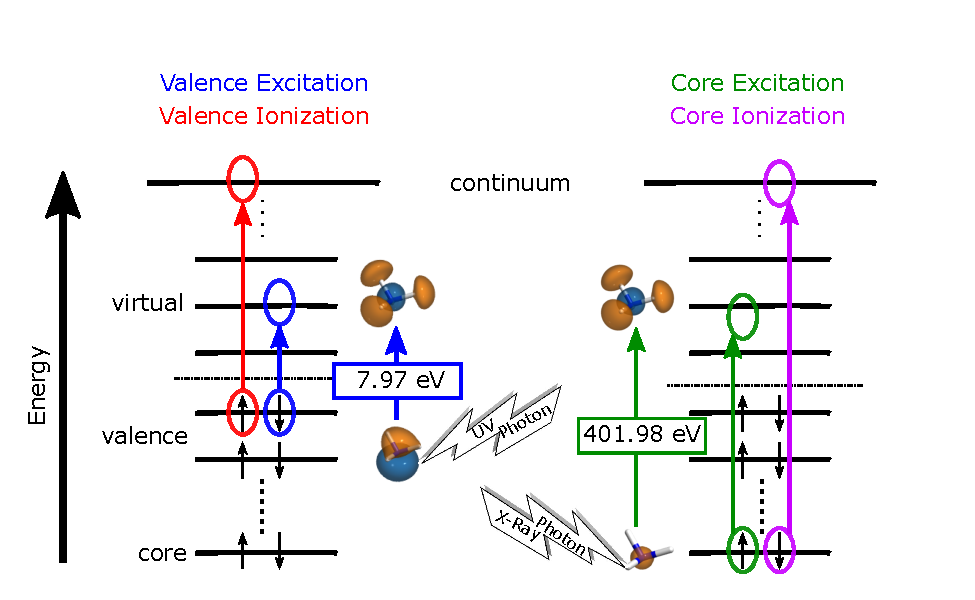
\includegraphics[scale=0.7]{photochem_graphic.pdf}
\caption{Sketch of the difference between UV and X-ray photo-absorption. The energies are not true to scale. The valence excitation and valence ionizaton processes are shown in blue and red respectively. The core excitation and core ionization processes are shown in green and purple respectively. An example is shown of the first valence and core excited state in ammonia (NH$_3$), the orbitals shown are hole and particle from orthogonality constrained density functional theory excited state computations at the B3LYP/3-21G level of theory.}
\label{fig:photochem}
\end{figure}

If we consider a closed-shell molecule, i.e. where all electrons are paired, when this molecule is not under the influence of any external radiation it is in its ground electronic state (S$_0$). Photons from impending radiation can excite the molecule from the ground state to an electronic excited state, promoting an electron from an occupied molecular orbital (MO) to a higher energy unoccupied MO (often referred to as a ``virtual'' orbital in quantum chemistry). The excitation energy ($\omega$) of the electronic excited state will depend upon the energy of the impending radiation. The lifetime of these electronic excited states are extremely short compared to the lifetime of molecular vibrations and thus these states can often be modeled properly within the vertical Franck-Condon approximation \cite{franck_elementary_1926,condon_theory_1926,condon_nuclear_1928,hazra_first_2004} where the electronic transition is assumed to occur without significant changes to the positions of the nuclei of the molecular system. The molecule eventually relaxes back down to its ground state level via a subsequent decay process such as fluoresence, \cite{maxwell_chlorophyll_2000,valeur_molecular_2012} phosphorescence, \cite{tanaka_observation_2005,romanovskii_phosphorescence_2000,cavar_fluorescence_2005} non-radiative relaxation, \cite{callomon_non-radiative_1972,de_mello_donega_non-radiative_1995} intersystem crossing, \cite{lamola_mechanisms_1965,hauser_intersystem_1991} and a myriad of other processes. \cite{zakrzewski_threshold_1984,meskers_relaxation_2000,vant_hof_zero-field_1976,hors_cross-relaxation_1982}

A unique class of electronic photo-excitations involves promotion of a core electron to a valence MO, the corresponding state is often referred to as core-excited (core-excited states). The electrons that constitute the ``core'' of a molecule are those occupying the lowest energy molecular orbitals. These MOs are not actively involved in bonding with the surrounding molecular environment and have orbital character similar to free-atom atomic orbitals (i.e. the 1s core orbital of NH$_3$ in Figure \ref{fig:photochem}). The number of MOs that compose the core is dependent upon the atomic number ($Z$) of the atom involved. For example, for lighter first-row elements in the periodic table, like oxygen, the 1s orbital is the only core orbital. However for heavier elements, like titanium, the 2s and 2p are also considered in the core level. Strong attractive Coulombic forces between the core electrons and the nuclei result in a large amount of energy being required to promote electrons from core levels. Thus, while ultraviolet (UV) or visible (VIS) photons are sufficient to excite valence electrons, high energy X-ray photons are required in order to excite core electrons. Figure \ref{fig:photochem} shows this process for both the valence and core cases respectively, and details the energy difference between the two in an example case of ammonia (NH$_3$). The first electronic valence excitation in ammonia has an excitation energy of 7.97 eV, meanwhile the first N core excitation has an excitation energy of 401.98 eV. It is clear that the high energy range, and unique nature of these transitions warrants an entire field of spectroscopy dedicated to its understanding.

\section{X-Ray Absorption Spectroscopy}
Core-excited states can be probed experimentally via X-ray absorption spectroscopy (XAS), a rapidly growing field that commonly makes use of synchrotron radiation in order to provide a tunable and intense X-ray beam source.\cite{snigirev_compound_1996,holch_new_2011} Tunability of the X-ray beam source allows it to scan a wide energy range throughout the X-ray region. Due to the large degree of energetic separation between the core and valence orbitals,\cite{politzer_separation_1976} scanning the X-ray beam through the binding energy of a core electron results in an abrupt increase in the absorption cross-section. This generates the so-called absorption ``edge'', with each unique edge region corresponding to a different core electron binding energy.\cite{stohr_nexafs_1992} The different edge regions are named using standard X-ray notation which is based on the principal quantum number of the excited electron; K for $n$=1, L for $n$=2, and M for $n$=3 (see Figure \ref{fig:xas_schematic}a).\cite{penner-hahn_x-ray_1999} Each edge is well separated from the rest of the absorption spectrum due to the dependence of the binding energy of core electrons on the charge of the nucleus. The fact that the edge position is dependent upon the atomic number ($Z$), XAS is often referred to as an ``element specific'' technique. For example, a typical K-edge resulting from oxygen core excitations is located at approximately 530 eV,\cite{yoon_oxygen_2002,parent_structure_2002} while the K-edge for nitrogen is located at approximately 400 eV.\cite{lambrecht_x-ray_1997,leinweber_nitrogen_2007} The existence of an absorption edge by itself has little relevance outside of simple elemental identification.\cite{cotte_synchrotron-based_2010} Fortunately the edge is not simply a discontinuous absorption increase, it has an abundance of structure (often referred to as ``fine structure'') throughout the different regions of the edge. Figure \ref{fig:xas_schematic}b shows a schematic drawing of a typical K-edge with the different regions of the fine structure highlighted. The first region of fine structure just before the edge is known as the pre-edge region. Although some organic 1s$\rightarrow$ $\pi^*$ transitions can populate this region, distinct features only arise in the case of transition metal complexes, where this region is populated by core transitions to unoccupied d-orbitals.\cite{yamamoto_assignment_2008,vedrinskii_pre-edge_1998,groot_1s_2009,roemelt_manganese_2012} The rising-edge region is composed of all other discrete core transitions of the system and has a distinct shape, that is typically dominated by intense 1s $\rightarrow$ $\pi^*$ transitions accompanied by weaker 1s $\rightarrow$ $\sigma^*$ transitions. The study of the fine structure that composes these two edge regions are the focus of near-edge X-ray absorption fine structure spectroscopy (NEXAFS).\cite{stohr_nexafs_1992} The last region of edge structure, the extended-edge region, is composed of signals past the ionization threshold of the core orbital in which core electrons are promoted to continuum (see Figure \ref{fig:photochem}). At this point the excited photoelectron has a high amount of energy, enough for its wavelength to be on the scale of interatomic distances. The resulting spectrum is a characteristic pattern of modulating local maxima and minima that correcpond to constructive and destructive interference between outgoing and backscattered photoelectron waves. As a result of this atomic-level sensitivity of the signal this region is sensitive to the radial distribution of electron density around the atom. The study of this signal, and its use to quantify geometric information such as bond lengths/coordination numbers is known as extended-edge X-ray absorption fine structure spectroscopy (EXAFS). \cite{lengeler_extended_1980,teo_exafs:_2012,gurman_rapid_1984,bunker_application_1983}

\begin{figure}
\centering
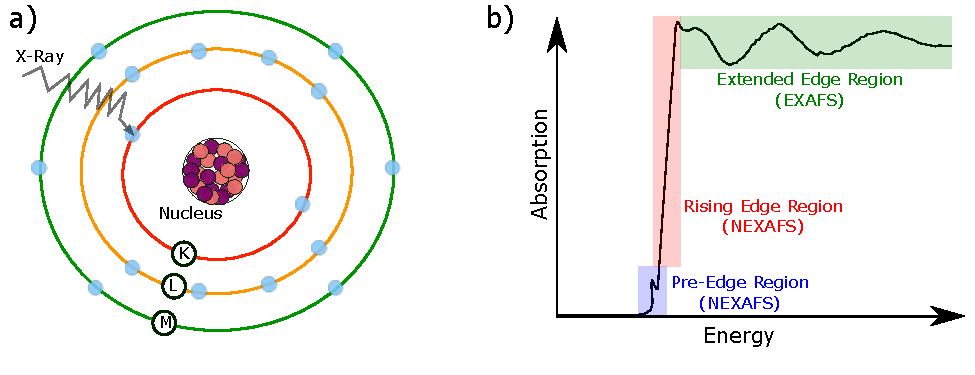
\includegraphics[scale=0.93]{XAS_schematic.pdf}
\caption{a) Schematic highlighting the X-ray absorption process, specifically shown here is an excitation of an electron from the first orbital shell (K-shell) of an arbitrary molecule. b) Drawing of the general shape of a K-edge X-ray absorption spectrum. The unique regions of the spectrum are marked and grouped with their corresponding spectroscopic method, either near-edge (NE) or extended-edge (E) x-ray absorption fine spectroscopy (XAFS).}
\label{fig:xas_schematic}
\end{figure}

With regard to the electronic structure of molecules, the near-edge region contains very useful information. \cite{garino_determination_2014,tourillon_electronic_1988} NEXAFS has been applied to a wide range of molecular systems including biological systems,\cite{zubavichus_nexafs_2004, zubavichus_nexafs_2009,samuel_nexafs_2017} small gas phase molecules,\cite{contini_gas-phase_2001,domke_carbon_1990,hudson_high-resolution_1994} organic thin-films,\cite{roy_structure_2005,hahner_near_2006,baldo_excitonic_1999} and semiconducting materials.\cite{guo_electronic_2011} For example, information regarding the orientation of organic molecules chemisorbed to surfaces can be obtained with NEXAFS. \cite{hoffmann_discovery_1990,stohr_bonding_1983,temprano_1d_2015,rastgoo-lahrood_post-synthetic_2016} One study investigated the adsorption structure of pyrazine (C$_4$H$_4$N$_2$) on a reconstructed Si(100) surface. \cite{lee_selective_2012} Through investigating changes in the polarization dependent NEXAFS spectrum, the geometry of the molecule relative to the surface normal could be deduced. NEXAFS can even be useful in explaining reaction mechanisms by using time-resolved X-ray spectroscopy.\cite{chen_probing_2005} A recent work by Attar et al. made use of time-resolved femtosecond NEXAFS in order to study the electrocyclic ring-opening reaction of 1,3-cyclohexadiene. \cite{attar_femtosecond_2017} Tracking the changes in the NEXAFS spectrum over time revealed strong mixing amongst the frontier orbitals and provided justification for the long postulated Woodward-Hoffman rules for pericyclic reaction mechanisms. \cite{day_aromaticity_1975}
Detailed interpretation of experimental X-ray absorption spectra requires knowledge of the relevant core excitation energies and excited state properties. Accurate quantum chemistry methods can often calculate electronic excited states and simulate the absorption spectrum of molecules. Along with interpretation of the properties and character of the transition, quantum chemistry calculations can yield plenty of useful information regarding the nature of electronic excited states. Many modern computational techniques have the capability of producing quantitatively accurate results regarding the excited states of systems of moderate size (less than 20 atoms). \cite{baeck_ab_2003,gwaltney_coupled-cluster_1998,shih_ab_1976,isborn_excited-state_2011} However, for the excited states of significantly larger systems, approximations must be made that represent a concession of accuracy for the sake of computational efficiency. \cite{fantacci_absorption_2003,de_angelis_electronic_2006} Utilizing quantum chemistry methods for the study of core-excited states encounters quite a few unique challenges. The most practical challenge they face from a purely computational perspective focuses on the eigenvalue solvers employed by many methods. Iterativive diagonalization algorithms are routinely employed as the eigenvalue solver in many quantum chemistry methods. \cite{gwaltney_simplified_1996,roos_new_1972,nakatsuji_structure_2001,mazur_application_2009} These approaches typically yield the lowest eigenvalue solutions and thus, tend to be efficient approaches for solving valence excited states. Core-excited states however, are much higher in energy. In order obtain solutions from the core region of the excitation spectrum, all underlying valence excited states must be calculated,\cite{imamura_time-dependent_2006} this is computationally inefficient in all cases and impossible for larger systems. Multiple strategies exist to overcome this algorithmic challenge, they typically revolve around target specific energy solutions \cite{besley_time-dependent_2010,peng_energy-specific_2015,lestrange_calibration_2015} or formally decoupling the space of core excitations from the space of valence excitations.\cite{ehlert_quest_2017,wenzel_calculating_2014} Both routes are viable options for overcoming this difficulty and the details of these approaches will be reviewed throughout the following section. Other challenges faced by quantum chemistry methods when calculating core-excited states are more physical in nature and have to do with the unique physics present in the core excitation mechanism. As stated previously, core electrons are tightly bound due to their close proximity to the nuclei and generation of a core hole causes significant orbital relaxation and a subsequent lowering of the total energy. Although orbital relaxation technically occurs in every excited state, the effect is less pronounced in valence excitations and is often times negligible in these calculations. To highlight this, a study by Triguero et al. \cite{triguero_separate_1999} investigated the sources of error in Koopmans approximation\bibnote{In Koopmans theorem the $i^{\rm th}$ Ionization potential is approximated by the corresponding energy eigenvalue of the canonical SCF equation $-\epsilon_i$.} of an ionization potential, . This error can be divided into three contributions: $R1$ ($<0$) due to orbital relaxation, $R2$ ($>0$) due to correlation,  and $R3$ ($<0$) due to the relaxation induced change in correlation. For valence ionizations, the relationship between the three sources of error is $-R1 \approx R2 \gg -R3$. However, for core ionizations this relationship becomes $-R1 \gg R2 \approx -R3$ with the error due to orbital relaxation becoming the dominant term. For example, Plakhutin et al. \cite{plakhutin_koopmans_2006} showed that for core ionization a nitrogen atom, $R1$ is on the order of 12-15 eV. \cite{plakhutin_koopmans_2006} Clearly this energy contribution is non-neglible for core-excited states and any quantum chemistry method striving for accurate energy calculations must consider this effect. Another consideration is the treatment of relativistic effects. Relativistic contraction of the core orbitals toward the nuclei results in a lowering of the core orbital energy while the valence orbital energies remain relatively uneffected. This results in an increase in excitation energy with respect to a nonrelativistic solution that is often non-negligible and becomes particularly important for core-excited states of heavier nuclei. 
\begin{table}
\centering
\caption{Non-relativistic (NR) and relativistic (R) energies (in eV) of the lowest lying core orbital and lowest unoccupied molecular orbital (LUMO) of water (H$_2$O) and silane (SiH$_4$) molecules calculated using spin-unrestricted Hartree--Fock (UHF) with the 3-21G basis set. Scalar relativistic effects are included by use of the 2$^{\rm nd}$ order Douglas-Kroll-Hess Hamiltonian.\cite{reiher_douglaskrollhess_2006} All calculations were performed using the ORCA software package.}
\begin{tabular}{ccccc}
\toprule
& \multicolumn{2}{c}{H$_2$O} & \multicolumn{2}{c}{SiH$_4$} \\ \cmidrule(lr){2-3} \cmidrule(lr){4-5}
& O 1s & LUMO & Si 1s & LUMO \\
\hline
NR-UHF & $-$555.88 & 7.17 & $-$1858.20 & 5.02\\
R-UHF & $-$556.34 & 7.16 & $-$1863.04 & 5.03\\
\bottomrule
\end{tabular}
\label{tab:rel_effects}
\end{table}
Table \ref{tab:rel_effects} shows orbital energies of the lowest lying core orbital and the lowest unoccupied molecular orbital (LUMO) for water (H$_2$O) and silane (SiH$_4$) molecules in a non-relativistic SCF calculation and a relativistic computation where scalar relativistic effects are taken into account using the Douglass--Kroll Hess Hamiltonian.\cite{reiher_douglaskrollhess_2006} The core orbital energy in H$_2$O lowers by 0.46 eV while the LUMO experiences negligible energy lowering of 0.01 eV. This effect becomes more pronounced with heavier elements, as the core orbital of silane experiences a relativistic contraction of 4.84 eV while it's LUMO raises in energy by only 0.01 eV. In the following section I will review the current theoretical approaches that have been applied to core-excited states and address how they approach the treatment and/or approximation the necessary components.

\section{Theoretical Approaches for Calculation of Core Excited States}
In the past, approaches for treatment of core-excited states were rare due to a lack of attention on XAS, however the advent of synchrotron radiation made these experiments more abundant and drove development throughout the years. This has lead to numerous computational approaches for calculating the properties of core-excited states. As discussed in detail in the previous section, core-excited states encounter a wealth of computational challenges including the algortihmic challenge of targeting the core region of the excitation spectrum and treatment of orbital relaxation and relativistic effects. This section will focus on reviewing theoretical approaches for the treatment of core-excited states within the framework of Hartree--Fock static exchange (HF-STEX),\cite{agren_direct_1994,hunt_excited_1969,zhang_nonlinear_2014,agren_direct_1997} time-dependent density functional theory (TDDFT), \cite{imamura_time-dependent_2006,besley_time-dependent_2007,lestrange_calibration_2015} and coupled cluster theory (CC).\cite{fransson_carbon_2013,besley_equation_2012,coriani_coupled-cluster_2012,coriani_asymmetric-lanczos-chain-driven_2012,myhre_near-edge_2016} For information regarding other noteworthy theoretical approaches including algebraic diagrammatic construction (ADC),\cite{wenzel_calculating_2014,wenzel_analysis_2015,wenzel_calculating_2014,wenzel_physical_2016} restricted active space self-consistent-field approaches (RASSCF),\cite{mochizuki_hf-stex_2001} configuration interaction,\cite{maganas_combined_2014,maganas_l-edge_2014,grimme_density_1996,asmuruf_calculation_2008} real-time time-dependent DFT (RT-TDDFT), \cite{lopata_linear-response_2012} and/or approaches using the Bethe-Salpeter equation,\cite{olovsson_near-edge_2009,vinson_theoretical_2012} I refer the reader to the existing literature on these topics. The focus here will be on treatment core-excitations relevant to K-edge applications, it is worth noting that there are numerous appraoches for the L-edge requires a more detailed theoretical treatment due to spin-orbit coupling,\cite{roemelt_combined_2013,ebert_l-edge_1996,maganas_first_2013} however this is outside of the scope of this dissertation. 

%A significant amount of progress has been made over the last few decades in order to make computations of core-excited states feasible and efficient in a plethora of different theories in quantum chemistry. As synchrotron facilities have become more powerful and plentiful the amount of high-quality X-ray absorption data has grown exponentially, inspiring more development in theory. Most modern techniques for the treatment of core-excitations fall into one of five classes that will be reviewed here: Hartree--Fock Static Exchange (HF-STEX), core valence separation (CVS), restricted excitation window (REW), energy specific (ES), or complex polarization propagator (CPP) methods. This review will focus primarily on methods used routinely in K-edge applications, there are more detailed multi-reference and relativistic methods in order to accurately treat the L-edge however those methods are outside the scope of this thesis. 
\subsection{Hartree-Fock Static Exchange}
HF-STEX (also known as improved virtual orbital Hartree--Fock) is a state specific Hartree--Fock approach in which a simplified configuration interaction singles expansion is performed to obtain excited states from a reference determinant that has been optimized for a core hole potential.\cite{agren_direct_1994,hunt_excited_1969,zhang_nonlinear_2014,agren_direct_1997} The reference determinant is constructed by performing an open-shell HF calculation in which an electron is removed from the core region of an N-electron system. Variational optimization of this (N$-$1)-electron state produces relaxed orbitals into the reference, providing an improved decription of the occupied and virtual HF orbitals. This direct inclusion of relaxation effects is one of the strongest advantages of HF-STEX based methods and is the starting approximation for practically every state specific/variational approach for core-excited state. The validity of this approximation supported by the large energy separation between the core and valence orbitals as well as the spatial separation of core orbitals on different atomic centers within a molecule. Let us consider an excitation from core orbital $j$ to valence orbital $b$ from a closed shell reference state $|\Psi_0\rangle$, the STEX eigenvalue problem can be defined as
\begin{equation}
\label{eq:HFSTEX_eig}
F^j \phi_b = \epsilon_{jb} \phi_b,
\end{equation}
where $F^j$ is the HF-STEX Fock operator
\begin{equation}
F^j = h + \sum_{i \neq j} (2J_i - K_i) + J_j - K_j.
\end{equation}
It should be noted that the excited states obtained from the open-shell HF reference are not orthogonal to the HF ground state and thus overlaps between the states must be accounted for. After accounting for non-orthogonality, the HF-STEX eigenvalue equation can be solved and the excitation energies ($\omega_{jb}$) can be obtained by adding the core ionization potential to the eigenvalue obtained in Equation \ref{eq:HFSTEX_eig}. The oscillator strengths are evaluated in terms of the excitation energy and the transition dipole moment as
\begin{equation}
f_{jb} = \frac{2}{3} \omega_{jb}|\langle \Psi_0|\vec{r}|\Psi_{jb}\rangle|^2,
\end{equation}
With regard to the performance of HF-STEX, it produces XAS spectra that are in acceptable quantitative agreement with experimental results. HF-STEX oscillator strengths also provide a good qualitative comparison with experimental line intensities.

Excited state solutions within HF-STEX can be best understood as an approximate solution to the random phase approximation (RPA).  Lets consider a general RPA excitation operator $\hat{T}_I$ for an excited state $I$ within the Tamm-Dancoff approximation (TDA):\cite{hirata_time-dependent_1999}
\begin{equation}
\hat{T}_I = \sum_{i,a} (\mathbf{X}_{ia,I}\hat{a}^{\dagger}_{a}\hat{a}_i),
\end{equation}
where $\mathbf{X}$ is the eigenvector of the RPA equation within the TDA, while $i$ and $a$ are indices that run over the ground state occupied and virtual orbitals respectively. This type of excitation operator contitutes what is known as a ``multi-channel'' approach, essentially a linear combination of single excitations that accounts for the interaction of different excitation channels. For HF-STEX, this excitation operator is limited to a restricted sum over single excitations from a given orbital $j$, also known as a ``single-channel'' approach
\begin{equation}
\hat{T}_I = \sum_{a} (\mathbf{X}_{ja,I}\hat{a}^{\dagger}_{a})\hat{a}_j,
\end{equation}
It should be noted that this would be an extremely poor approximation for valence-excited states as multiple excitation channels tend to be clustered within a fairly small energy range (potentially less than 1 eV). However, due to the large energy separation of core orbitals, it is possible to obtain an accurate simulation of the XAS spectrum within a single channel approximation. 

The attractive features of this theory are however hampered by two main challenges.  The first is the difficulty of converging the open-shell SCF reference state necessary to build the STEX Hamiltonian. It is notoriously difficult to converge on the desired core hole state. However, there are solutions to this problem that can aide convergence of the core hole state, most notably the maximum overlap method.\cite{besley_self-consistent-field_2009} The second challenge with HF-STEX lies in the non-orthogonality of the excited states within the core-hole potential which requires explicit wavefunction overlaps to be accounted for. 
\subsection{Linear Response Time-Dependent Density Functional Theory Approaches}
With regard to computational cost, linear response time-dependent density functional theory (TDDFT) remains one of the most attractive options for calculating electronic excited states in a wide variety of systems. Within TDDFT, excitation energies ($\omega$) are calculated via solutions to the following non-Hermitian eigenvalue equation:
\begin{equation}
\label{eq:tddft_eigenvalue_equation}
\begin{pmatrix}
\mathbf{A} & \mathbf{B} \\
\mathbf{B^{\dagger}} & \mathbf{A^{\dagger}} 
\end{pmatrix} 
\begin{pmatrix}
\mathbf{X}\\
\mathbf{Y}
\end{pmatrix}
= \omega
\begin{pmatrix}
\mathbf{1} & 0 \\
0 & -\mathbf{1}
\end{pmatrix}
\begin{pmatrix}
\mathbf{X} \\
\mathbf{-Y}
\end{pmatrix},
\end{equation}
where the matrices $\mathbf{A}$ and $\mathbf{B}$ are given by
\begin{align}
\label{eq:A_matrix}
A_{ai\sigma,bj\tau} &=  \delta_{ij} \delta_{ab} \delta_{\sigma\tau}(\epsilon_{a\sigma} - \epsilon_{i\tau}) + (ia\sigma|jb\tau) + (ia\sigma|f_{\rm XC}|jb\tau), \\
\label{eq:B_matrix}
B_{ai\sigma,jb\tau} &= (ia\sigma|jb\tau) + (ia\sigma|f_{\rm XC}|jb\tau),
\end{align}

for occupied orbitals $i,j,...$, virtual orbitals $a,b,...$, spin indices $\sigma$ and $\tau$, and energy eigenvalues $\epsilon$. The second term in Equation \ref{eq:A_matrix} is a two-electron integral and can be expressed explicitly in terms of a set of Kohn--Sham orbitals ($\phi_i$) as:

\begin{equation}
(ia\sigma|jb\tau) = \int \int \phi^*_{i\sigma}(\mathbf{r}_1)  \phi^*_{a\sigma}(\mathbf{r}_1) \frac{1}{r_{12}} \phi^*_{j\tau}(\mathbf{r}_2) \phi^*_{b\tau}(\mathbf{r}_2) d\mathbf{r}_1 d\mathbf{r}_2,
\end{equation}

while the third term is what is known as the exchange correlation kernel which can be expressed as the functional derivative

\begin{equation}
(ia\sigma|f_{\rm XC}|jb\tau) = \int \phi^*_{i\sigma}(\mathbf{r}_1)  \phi^*_{a\sigma}(\mathbf{r}_1) \frac{\delta^2 E_{XC}}{\delta \rho{\sigma}(\mathbf{r}_1 \delta \rho_{\tau}(\mathbf{r}_2)} \phi^*_{j\tau}(\mathbf{r}_2) \phi^*_{b\tau}(\mathbf{r}_2) d\mathbf{r}_1 d\mathbf{r}_2,
\end{equation}
where $E_{\rm XC}$ is the exchange correlation functional. Within the Tamm-Dancoff approximation (TDA),\cite{fetter_quantum_1971} Equation \ref{eq:tddft_eigenvalue_equation} reduces to a Hermitian eigenvalue equation $\mathbf{A}\mathbf{X} = \omega\mathbf{X}$. Eliminating the off diagonal elements $\mathbf{B}$ greatly reduces the computational cost of solving the equation and makes the theory formally similar to configuration interaction singles. Many modern implementations of TDDFT make use of some form of the Davidson algorithm which iteratively diagonalizes a subspace of the Hamiltonian yielding its lowest (highest) eigenvalues in a bottom-up (top-down) fashion. This is a reasonable and efficient choice when the excitations of interest are valence excitations. However, excitations involving the lower energy core orbitals introduce a significant computational challenge since there is typically a plethora of valence excitations below the target core excitations, making the algorithm prohibitively. Overcoming this prohibitive expense is the primary motivation of methods developed to calculate core excitations within the TDDFT. 
\subsubsection{Restricted Excitation Window TDDFT}
Originally proposed by Stener et al.,\cite{stener_time_2003} restricted excitation window TDDFT (REW-TDDFT) is a modification to the standard TDDFT algorithm that only allows electrons to be excited from a subset of core orbitals. \cite{imamura_time-dependent_2006,besley_time-dependent_2007} This approximation is physically motivated by the large energy separation of core levels of different atomic species, and the large spatial separation of core orbitals on different atoms. This is normally done in one of two ways: (1) Core orbitals of interest are selected directly via orbital localization schemes for equivalent atoms (i.e. selecting all MOs that have primarily oxygen 1s character) or (2) Use an orbital energy (energy difference) cutoff in order to filter out any orbitals (orbital pairs) that lie above (below) the user provided energy threshold. The latter option is by far the most popular and has become commonplace for TDDFT implementations in modern quantum chemistry packages. 

Although REW-TDDFT allows for the computation of core excited states, it naturally inherits the issues of standard TDDFT calculations, namely the large dependence on the choice of exchange-correlation functional. This has lead to development of a new class of functionals for use with REW-TDDFT known as short range corrected (SRC) functionals which are modified versions of long range corrected (LRC) functionals used for charge transfer excitations in TDDFT. The LRC exchange correlation functional can be expressed as
\begin{equation}
E^{\rm LRC}_{\rm XC} = E^{\rm SR-DFT}_{\rm X} + E^{\rm LR-HF}_{\rm X} + E^{\rm DFT}_{\rm C},
\end{equation}
combining a DFT exchange in the short-range ($E^{\rm SR-DFT}_{\rm X}$), with Hartree--Fock exchange in the longer-range ($E^{\rm LR-HF}_{\rm X}$), and DFT correlation energy ($E^{\rm DFT}_{\rm C}$). SRC functionals modify this general form to include a certain portion of Hartree--Fock exchange in the short range as well, where the SRC exchange-correlation energy ($E^{\rm SRC}_{\rm XC}$) can be expressed as
\begin{equation}
E^{\rm SRC}_{\rm XC} = c_{\rm X}E^{\rm SR-HF}_{\rm X} + E^{\rm SR-DFT}_{\rm X} + E^{\rm LR-HF}_{\rm X} + E^{\rm DFT}_{\rm C}, 
\end{equation}
where $c_{\rm X}$ is a parameter that can be optimized. The major drawback with this method is that the amount of HF exchange in the functional must be re-optimized for any given system, which can be cumbersome and limits its reliability in application to novel problems. 
\subsubsection{Energy Specific TDDFT}
Starting from the non-Hermitian eigenvalue problem shown in Equation \ref{eq:tddft_eigenvalue_equation}, this form is often placed into the following equivalent Hermitian eignvalue equation
\begin{equation}
(\mathbf{A} - \mathbf{B})^{1/2} (\mathbf{A} +\mathbf{B}) (\mathbf{A} - \mathbf{B})^{1/2} \mathbf{T} = \omega^2 \mathbf{T},
\end{equation}
where $\mathbf{T} = (\mathbf{A} - \mathbf{B})^{-1/2} (\mathbf{X} + \mathbf{Y})$. Energy Specific TDDFT (ES-TDDFT) \cite{lestrange_calibration_2015} aims to solve this Hermitian eigenvalue problem utilizing a ``growing window'' algorithm that starts from a set of trial vectors $\mathbf{C}$ associated with orbital pairs whose orbital energy difference are above a given threshold. A subspace $\mathbf{\tilde{M}}$ is then created using the trial vectors,
\begin{align}
\mathbf{\tilde{M}}^+ &= \mathbf{C^T} (\mathbf{A} +\mathbf{B})\mathbf{C} \\
\mathbf{\tilde{M}}^- &= \mathbf{C^T} (\mathbf{A} -\mathbf{B})\mathbf{C} \\
\mathbf{\tilde{M}} &= (\mathbf{\tilde{M}} ^-)^{1/2} (\mathbf{\tilde{M}} ^+) (\mathbf{\tilde{M}}^-)^{1/2},
\end{align}
Direct diagonalization is performed only in the subspace $\mathbf{\tilde{M}}$, which generates a new set of eigenvalues $\tilde{\omega}$ and eigenvectors $\tilde{T}$. Only those eigenvectors associated with eigenvalues above the user defined threshold are kept. These eigenvectors are then projected back onto the full MO space in order to calculate a residual, any new eigenvectors with significant amplitude are then added as a trial vector for the next iteration (hence the term ``growing window''). A new subspace is constructed from the expanded trial space and the process continues self-consistently until the residual is below a user-defined threshold.

Since this method checks the residual of the subspace against the full MO space, the final results that are obatained are true solutions of the TDDFT equations. Similar to REW-TDDFT, however, it inherits the functional dependence of TDDFT for the calculation of core excited states.

\subsection{Coupled Cluster Approaches}
The coupled-cluster wavefunction ($\Psi_{\rm CC}$) can be defined as an exponential expansion of a closed 
shell HF reference ($\Psi_{\rm HF}$)
\begin{equation}
|\Psi_{\rm CC}\rangle = e^{\hat{T}}|\Psi_{\rm HF} \rangle,
\end{equation}
where $\hat{T}$ is known as the cluster operator can be expressed as a linear combination of single, double, triple, etc. excitations, up to N-fold excitations for a general N-electron system
\begin{equation}
\hat{T} = \hat{T}_1 + \hat{T}_2 + \hat{T}_3 + ... + \hat{T}_N.
\end{equation}
Where each individual excitation operator is composed of cluster amplitudes ($t_{\mu}$) and excitation operators ($\hat{\tau}_{\mu}$) that represent excitations from occupied orbitals (i,j,k,...) to virtual orbitals (a,b,c,...)
\begin{equation}
\hat{T} = \sum_{\mu} t_{\mu} \hat{\tau}_{\mu} = \sum^{\rm occ}_{i > j > k> ...} \sum^{virt}_{a > b > c > ...} t^{abc...}_{ijk...} \hat{\tau}^{abc...}_{ijk...}.
\end{equation}
The total energy (E) and amplitudes ($\Omega_{\mu}$) of the ground state can then be determined by projections onto the reference state and onto a manifold of excitations out of the reference state
\begin{align}
E &= \langle \Psi_{\rm HF} | e^{- \hat{T}}\hat{H} e^{\hat{T}} |  \Psi_{\rm HF} \rangle, \\
\Omega_{\mu} &= \langle \Psi_{\mu} | e^{- \hat{T}}\hat{H} e^{\hat{T}} |  \Psi_{\rm HF} \rangle = 0.
\end{align}
The truncation of the cluster operator $\hat{T}$ gives rise to the different ``levels'' of coupled cluster theory:
\begin{align}
{\rm CCS}&: \hat{T}_1 \\
{\rm CCSD}&: \hat{T}_1 + \hat{T}_2 \\
{\rm CCSDT}&: \hat{T}_1 + \hat{T}_2 + \hat{T}_3 \\
{\rm CCSDTQ}&: \hat{T}_1 + \hat{T}_2 + \hat{T}_3 + \hat{T}_4  \\
\nonumber
\vdots
\end{align}
Within coupled-cluster theory, excited states can be obtained via a linear-response approach as well as a state-specific approach. Both approaches have challenges that must be overcome in order to calculate core-excited states. These methods for calculating core-excited states will be reviewed here.
\subsubsection{Linear-Response Coupled Cluster Theory}
Within coupled-cluster linear response theory,(CC-LR) excitation energies ($\omega_{k}$) are obtained by solving an asymmetric eigenvalue equation to obtain right ($\mathbf{R}_k $) and left ($\mathbf{L}_k$) eigenvectors, commonly referred to as excitation and de-excitation operators respectively
\begin{align}
\label{eq:right_cc}
\mathbf{AR_k} &= \omega_k \mathbf{R_k}, \\
\label{eq:left_cc}
\mathbf{L_kA} &= \omega_k \mathbf{L_k},
\end{align}
where the left and right eigenvalues are orthogonal ($\mathbf{L_iR_k} = \delta_{ik}$), and A is a Jacobian matrix that is defined as the gradient of the cluster amplitudes
\begin{equation}
A_{\mu \nu} = \frac{\partial \Omega_{\mu}}{\partial t_\nu},
\end{equation}
Many general schemes to iteratively solve Equations \ref{eq:right_cc} and \ref{eq:left_cc} have been introduced for excited state calculations. These methods typically rely on using HF orbital energy differences to select guess unit vectors for specific occupied to virtual excitations. One fatal flaw that many methods encounter when trying to calculate core-excitations, is that the iterative solver will converge onto the lowest energy eigenvalues and eigenvectors even if the starting unit vectors are chosen for higher energy excitations. To overcome this difficulty, Coriani and Koch introduced a novel approach to iteratively solving Equations \ref{eq:right_cc} and \ref{eq:left_cc} using an asymetric Lanczos algorithm.\cite{coriani_coupled-cluster_2012,coriani_asymmetric-lanczos-chain-driven_2012} This approach employs a tridiagonal representation $\mathbf{T}$ of the Jacobian matrix $\mathbf{A}$. 
\begin{equation}
\mathbf{T} = \mathbf{P^T A Q},
\end{equation}
where $\mathbf{P^TQ} = \mathbf{1}$. The diagonalization of $T$ is truncated at a dimension that is greatly reduced compared to the full dimension of possible excitations, generating an effective excitation spectrum. Using this approach the excitation spectrum converges to the exact excitation spectrum from the bottom or the top, i.e. higher energy starting vectors do converge on the higher energy. 
\subsubsection{Equation-of-Motion Coupled Cluster Singles and Doubles}
Within the context of EOM-CCSD, it is conveniant to define a normal ordered Hamiltonian ($H_N$) that can be defined as
\begin{equation}
\hat{H}_N = e^{-\hat{T}}\hat{H}e^{\hat{T}} - E,
\end{equation}
this normal ordered Hamiltonian is then used to build the matrix elements of the EOM-CCSD Hamiltonian 
\begin{align}
\nonumber
\hat{H}_{\rm EOM-CCSD} &= 
\begin{bmatrix}
\hat{H}^{\rm SS} & \hat{H}^{\rm SD} \\
\hat{H}^{\rm DS} & \hat{H}^{\rm DD}
\end{bmatrix} \\
\nonumber
\hat{H}^{\rm SS} &= \langle \Phi_{i}^{a} | \hat{H}_N | \Phi_{k}^{c} \rangle \\
\nonumber
\hat{H}^{\rm SD} &= \langle \Phi_{i}^{a} | \hat{H}_N | \Phi_{kl}^{cd} \rangle \\
\nonumber
\hat{H}^{\rm DS} &= \langle \Phi_{ij}^{ab} | \hat{H}_N | \Phi_{k}^{c} \rangle \\
\hat{H}^{\rm DD} &= \langle \Phi_{ij}^{ab} | \hat{H}_N | \Phi_{kl}^{cd} \rangle,
\end{align}
where $|\Phi_{i}^{a} \rangle$ and $|\Phi_{ij}^{ab} \rangle$ are the singly and doubly excited determinants respectively. This EOM-CCSD Hamiltonian is then diagonalized using a modified Davidson algorithm to obtain the excitation energy eigenvalue spectrum. Similar to CC-LR, EOM-CCSD suffers from a feasibility problem as the high energy core-excited states can only be obtained after first obtaining a series of lower energy solutions. The need to solve for the full dimension of excitations in order to reach the core-excited states of interest causes standard diagonalization techniques to become computationally expensive for all cases and impossible for reasonably large cases. This issue can be handled in a similar way to the energy specific TDDFT method outlined above, to yield an energy specific EOM method (ES-EOM-CCSD)\cite{peng_energy-specific_2015}

\begin{comment}
\subsection{Real-Time Time-Dependent Density Functional Theory}
An alternative time-dependent density functional theory approach is real-time TDDFT (RT-TDDFT). In RT-TDDFT the density matrix is propagated in time utilizing the time dependent form of the Kohn-Sham equation. [CITE] This is done by solving the following equation of motion
\begin{equation}
\label{eq:real_time_EOM}
i \frac{\partial \mathbf{D}(t)}{\partial t} = [\mathbf{F}(t), \mathbf{D}(t)]
\end{equation}
where $\mathbf{D}(t)$ is the time dependent one-electron density matrix and $\mathbf{F}(t)$ is the time dependent Fock matrix which can be expressed in the following form for the case of hybrid exchange-correlation functionals
\begin{equation}
\label{eq:time_dependent_fock}
\mathbf{F}[\mathbf{D}(t)] = \mathbf{H}^{\rm core} + \mathbf{J}[\mathbf{D}(t)] + \mathbf{E}_{\rm XC} [\rho(\mathbf{r},t)]- \mathbf{\mu} \mathbf{V}^{\rm ext}(t)
\end{equation}
where $\rho(\mathbf{r}, t)$ is the time-dependent electron density, $\mathbf{\mu}$ is the dipole matrix, and $\mathbf{V}^{\rm ext}(t)$ is the applied external potential. The coefficients $\alpha$, $\beta$, and $\gamma$ are parameters that control the amount of Hartree--Fock and DFT exchange, respectively. It should be noted that the expression in Equation \ref{eq:time_dependent_fock} only considers the coupling of the dipole moment with the external potential, this is valid within the ``long wavelength'' approximation where it is assumed that the photon is much longer than the system size. This approximation is almost always valid for UV/Vis photons and X-ray photons of organic molecules, however, it can breakdown for higher energy core excitations in transition metals. At which point it will be necessary to consider higher order multipole moments beyond the electric dipole approximation. [CITE]

Solutions to the real-time approach involve integrating Equation \ref{eq:real_time_EOM} in order to obtain the time-dependent density matrix.  The Magnus expansion is a popular integrator for obtaining these solutions. [CITE] Within this expansion the density matrix is propagated through time via a unitary propagator which conserves idempotency. The exact unitary propagator for Equation \ref{eq:real_time_EOM} is given as
\begin{equation}
\mathbf{U}(t + \Delta t, t) = T \ {\rm exp}\{-i \int^{t+\Delta t}_t \mathbf{F}(\tau) d\tau\},
\end{equation}
such that the time propagation of the density matrix can be written as
\begin{equation}
\mathbf{D}(t + \Delta t) = \mathbf{U}(t + \Delta t, t) \mathbf{D}(t) \mathbf{U}^{\dagger}(t + \Delta t, t),
\end{equation}
where $\Delta t$ is the time-step and $T$ is a time-ordering operator that orders the operations associated with later times from those associated with earlier times. Due to the explicit time dependence of the Fock matrix it is impossible to evalute this propagator directly. However, it can be written in terms of a Magnus expansion
\begin{equation}
 T \ {\rm exp}\{-i \int^{t+\Delta t}_t \mathbf{F}(\tau) d\tau\} = e^{\Omega_1 + \Omega_2 + ... +\Omega_M},
\end{equation}
where $M$ is the total number of Magnus terms $\Omega_i$. The Magnus expansion is typically truncated at $M=1$ such that the unitary propagator can be approximated as
\begin{align}
\mathbf{U}(t + \Delta t, t) &\approx e^{\Omega_1} \\
\Omega_1 &\approx -i\mathbf{F}(t + \Delta t/2).
\end{align}
Within this form, the Fock matrix at a future time is guessed via linear extrapolation and solved for iteratively. This allows for the following explicit form of the time propagation of the density matrix
\begin{equation}
\mathbf{D}(t + \Delta t) = e^{-i\mathbf{F}(t+\Delta t/2)\Delta t} \mathbf{D}(t) e^{-i\mathbf{F}(t+\Delta t/2)\Delta t}.
\end{equation}
Core excitations typically have oscillations on the attosecond timescale, thus time steps on the tenth of an attosecond time scale must be taken to ensure accuracy within this region. An optical absorption spectrum can be obtained from a real-time simulation via a Fourier transform of the time-dependent dipole moment that results from a small applied electric field. For excitations on longer time scales, a Gaussian electric field can be chosen, however to accomodate the short time scales of core excitations a delta function perturbation is typically applied [CITE]
\begin{equation}
\mathbf{E}_{\delta}(t) = \kappa \delta(t) \mathbf{\hat{d}}.
\end{equation}
\end{comment}
%\subsection{Theoretical Treatment of X-Ray Absorption Spectroscopy}
%Our starting point for an introduction to the theory of XAS is the simplification of the many electron problem into a generalized independent particle approximation based on the standard hole/electron quasiparticle picture. This simplifies the many-body theory into an effective independent electron approximation of an electronic excitation from initial state $|i\rangle$ to final state $|f\rangle$. Within this simplified picture, the absorption coefficient $\mu$ for a given photon energy $\omega$ can be expressed as
%\begin{equation}
%\mu(\omega) \approx \sum_f | \langle i | d | f \rangle |^2 \delta(\hbar \omega + E_i - E_f)
%\end{equation}
%where $\hbar \omega + E_i$ is the energy of the photoelectron and $d$ is the dipole coupling to the x-ray field. This equation is essentially a sum over final states $|f\rangle$. The composition of the final states are important to the theory and must provide an accurate representation of the excited state, however their construction in this case is not obvious. Many modern one-electron theories construct the final states in a self-consistent potential that includes a core-hole, this procedure is known as the Hartree--Fock static exchange approximation (HF-STEX). This approximation is physically motivated by the large energy separation of core levels of different atomic species, and the large spatial separation of core orbitals on different atoms. Allowing for a single excitation to be modeled in terms of relaxed orbitals from a given core-hole state. Within this approximation, $\psi_f$ is the wavefunction representing the final state with $h^{\prime}$ as the Hamiltonian of the core-hole potential, yielding the following eigenvalue equation
%\begin{equation}
%h^{\prime} \psi_f = E \psi_f
%\end{equation}
%where E represents the final state energies, and $h^{\prime}$ has the following form
%\begin{equation}
%h^{\prime} = \frac{p^2}{2m} + V^{\prime}_H + \sum(E)
%\end{equation}
%where the first term is the kinetic energy, $V^{\prime}_H$ is the Hartree potential of the core-hole state and $ \sum(E)$ is the self-energy term. This quantity is a complex valued, dynamically screened exchange interaction that accounts for the many body effects of extrinsic loses that occur due to the propagation of the photoelectron. $ \sum(E)$ is analogous to the exchange correlation potential of density functional theory, essentially containing all information not captured in the kinetic and potential term. Within GW theory, $ \sum(E)$ has been effectively approximated and provides accurate results for EXAFS spectroscopy. However, this term is overestimated for near-edge applications and thus further treatment is necessary.
%\subsection{Near-Edge X-ray Absorption Fine Structure}
%As with any form of photo-electron spectroscopy the interpretation of XAS spectroscopy relies on the Beer-Lambert law which relates the exponential decrease of the intensity ($I$) of the transmitted beam with respect incident beam intensity ($I_0$):
%\begin{equation}
%I = I_0 e^{-\mu D}
%\end{equation}
%where $D$ is the sample thickness and $\mu$ is what's known as the linear absorption coefficient which is related to the absorption cross-section, $\sigma_i$, of the $n$ unique chemical elements present in the sample
%\begin{equation}
%\mu = \frac{1}{V} \sum^n_{i = 1} \sigma_i
%\end{equation}
%where $V$ is the volume of the sample. Interpretation of the spectrum requires analysis of the position, intensity, and spape of peak features. As stated earlier, the position of peak features an energy specific signature of the absorbing atom. However, the technique is sensitive enough to differentiate between the same element in unique chemical environments.
%\begin{figure}
%\centering
%\includegraphics[scale=0.5]{chromium_k_edge.png}
%\caption{NEXAFS spectra at the Cr K-edge of four unique Cr(III) containing compounds. Experimental spectra are shown as solid lines, theoretical spectra are shown as dotted lines and are calculated using multiple scattering theory inside the FEFF8 code.[CITE] All data is from ref [CITE]}
%\label{fig:chromium_k_edge}
%\end{figure}
%For example, Figure \ref{fig:chromium_k_edge} shows the different spectra for four different Cr(III) containing metal complexes. Although all of the Cr K-edge spectra appear in the same region (5980 - 6050 eV), each unique complex has a different spectral profile in terms of peak positions and lineshapes. This shows that NEXAFS is sensitive to differences in the electronic structure, even the structurally similar CrF$_3$ and CrCl$_3$ have drastically different K-edge footprints. The same is true of atoms at different oxidation states, when increasing oxidation the edge tends to shift toward higher energy. This makes NEXAFS an excellent tool to check the valence state of atoms. 

%The K-edge, which consists of excitations of 1s electrons forms a rich structure for any atom that serves as a resource to interpret the unoccupied states of the electronic structure. The L-Edge is more complex to interpret, however is just as powerful in interpreting information about a molecules electronic structure. The complexity arises from the degeneracies that exist at the 2p electronic level, this introduces an element of strong electron correlation and causes splitting in the spectrum related to spin-orbit coupling between the occupied p-orbitals and unoccupied 3d states. 

\section{Orthogonality Constrained Density Functional Theory}
In this section, I review orthogonality constrained density functional theory (OCDFT) as a general approach to electronic excited states. OCDFT belongs to a unique class of density functional approaches whose main goal is to study excited states without using a time-dependent formulation, otherwise known as time independent density functional theory (TIDFT). \cite{samal_exploring_2006,ayers_time-independent_2009} This class of methods aim to provide an alternative to TDDFT which has been known to struggle in cases of charge transfer and Rydberg excited states due to inadequacies of approximate exchange correlation functionals. \cite{zhang_challenge_1998,cohen_insights_2008}

OCDFT is a variational formulation of DFT for the calculation of excited states.\cite{evangelista_orthogonality_2013} Unique to the theory is the explicit enforment of constraints that guarantee orthogonality while allowing the MOs to fully relax. This draws inspriation from two TIDFT theories: 
\begin{itemize}
\item The variational TIDFT approach of Levy and Nagy which provides the theoretical framework for a universal excited state density functional,\cite{ayers_time-independent_2012} thereby justifying the variational optimization of an excited state in DFT.
\item The constrained DFT (CDFT) approach of Van Voorhis and coworkers \cite{kaduk_constrained_2012} which provides a framework for studying systems within Kohn--Sham DFT that have an arbitrary constraint on their density.
\end{itemize} 
The remainder of this section will provide a brief introduction to the theory, following this introduction will be a discussion of the features of the theory that specifically make it an attractive choice for the calculation of core-excited states.
\subsection{Original Formulation via Constrained Variational Minimization}
Within a generalized Kohn--Sham (KS) framework, an $n$-electron system can be represented in terms of an auxiliary system of noninteracting electrons. \cite{hohenberg_inhomogeneous_1964,kohn_self-consistent_1965} The KS auxiliary system can be represented by a single Slater determinant 
\begin{equation}
|\Phi\rangle = | \phi_1, \phi_2, ..., \phi_n \rangle,
\end{equation}
which is constructed from a set of KS orbitals \{$\phi_i$\}. The total ground state electronic energy of the KS system can be expressed as
\begin{equation}
E_{\rm KS}[\{\phi_i\}] = - \frac{1}{2} \sum^{\rm occ}_i \langle \phi_i| \bigtriangledown^2 | \phi_i \rangle + \int d\mathbf{r} \nu(\mathbf{r}) \rho(\mathbf{r}) + J[\rho] + E^{\prime}_{\rm XC}[\rho],
\end{equation}
where the first term is the kinetic energy contribution, the second term is the contribution of the external potential, while $J[\rho]$ and $E^{\prime}_{\rm XC}[\rho]$ are the Coulomb and exchange-correlation contribution respectively. In general, an excited state can be computed by a constrained minimization of the expectation value of the Hamiltonian ($\hat{H}$) over all the wave funtions orthogonal to the ground state $\Psi$:
\begin{align}
E^{\prime} &= \min_{\rho^{\prime}}\left\{\min_{\substack{\Psi^{\prime} \rightarrow \rho^{\prime} \\ \Psi^{\prime} \perp \Psi}} \langle \Psi^{\prime}| \hat{H} | \Psi\rangle \right\} \\
&= \min_{\rho^{\prime}}\left\{ \int d\mathbf{r} \nu(\mathbf{r}) \rho(\mathbf{r}) + F^{\prime}[\rho^{\prime}]\right\},
\end{align}
where $F^{\prime}[\rho^{\prime}]$ minimizes the sum of the kinetric energy ($\hat{T}$) and electron-electron repulsion. In the spirit of the variational TIDFT of Levy and Nagy, OCDFT introduces a ficticious KS system of noninteracting electrons with density $\rho^{\prime}_s$ which maps to the excited state density of the real interacting system $\rho^{\prime}$ and can be described by a unique Slater determinant $\Phi^{\prime}$. The excited state solution is obtained via a \textit{constrained minimization} subject to an orthogonality constraint on the auxiliary wavefunctions
\begin{equation}
\langle \Phi^{\prime}|\Phi \rangle = 0,
\end{equation}
Direct imposition of this orthogonality constraint avoids the excited state wavefunction from collapsing to the ground state solution. The OCDFT energy functional for the excited state is then expressed as
\begin{equation}
E^{\prime}_{\rm OCDFT}[\{\phi^{\prime}_i\}] = - \frac{1}{2} \sum^{\rm occ}_i \langle \phi^{\prime}_i| \bigtriangledown^2 | \phi^{\prime}_i \rangle + \int d\mathbf{r} \nu(\mathbf{r}) \rho^{\prime}(\mathbf{r}) + J[\rho^{\prime}] + E_{\rm XC}[\rho^{\prime}],
\end{equation}
Note that the exchange-correlation functional $E_{XC}$ is approximated with the ground state functional evaluated at the excited state density. This is an adiabatic approximation for the excited state and is discussed in more detail in Ref. \citenum{evangelista_orthogonality_2013}. 
\subsection{Attractive Features of OCDFT for Core Excitations}
This section will focus on the features of orthogonality constrained density functional theory that make it an attractive candidate as a theory for core excitations. Three features stand out the most and will be covered in more detail in this section:
\begin{itemize}
\item Full inclusion of orbital relaxation effects through variational optimization of Kohn--Sham orbitals.
\item Variational stability of the $\Delta$SCF procedure due to imposition of orbital orthogonality.
\item Computational cost and scaling comparable to time-dependent density functional theory.
\end{itemize}
Having established itself as a stable, cheap, and accurate theory for electronic excited states the extension of this theory for the treatment of core excited states seemed like a logical progression.
\subsubsection{Orbital Relaxation Effects}
Within OCDFT, a general excited state determinant $\Phi^{\prime}$ for an $n$-electron system is optimized with respect to a set of excited state orbitals $\{\phi_n^{\prime}\}$ 
\begin{equation}
|\Phi^{\prime} \rangle = | \phi^{\prime}_1, \phi^{\prime}_2, ..., \phi^{\prime}_n \rangle,
\end{equation}
Since the excited state is variationally optimzed, relaxation effects are explicitly considered for each excited state determinant. Within a quasiparticle framework, two of the orbitals that compose this slater determinant will define the excitation process as the hole ($\phi^{\prime}_h$) and particle ($\phi^{\prime}_p$) respectively. The excited state orbitals are optimized subject to a set of minimal orbital orthogonality conditions: 1) The occupied orbitals are restricted to span the space complementary to the hole orbital 
\begin{equation}
\langle \phi^{\prime}_i|\phi_h^{\prime}\rangle = 0, i=1,2,...n
\end{equation}
and 2) The hole orbital must be constrained to span the occupied space of the ground state determinant $\Phi$. Optimizing the the excited state relative to these two constraints is sufficient to produce an orthogonal excited state solution. This formalism provides the flexibility to control the degree of optimization of the wavefunction, i.e. to control the amount of relaxation that it explicitly included in the calculation. This analysis was very useful for determining the importance of relaxation effects on the performance of OCDFT in valence excitations, \cite{evangelista_orthogonality_2013} and a similar analysis is applied here to examine the importance for core excitations. We make use of 3 different levels of optimization 1) Obtaining the fully optimal hole/particle pair and allowing full relaxation of all alpha and beta orbitals 2) Obtaining the optimal hole/particle pair while only allowing relaxation of the alpha orbitals 3) and Obtaining the optimal hole orbital only while allowing all other alpha/beta orbitals to relax
\begin{figure}
\centering
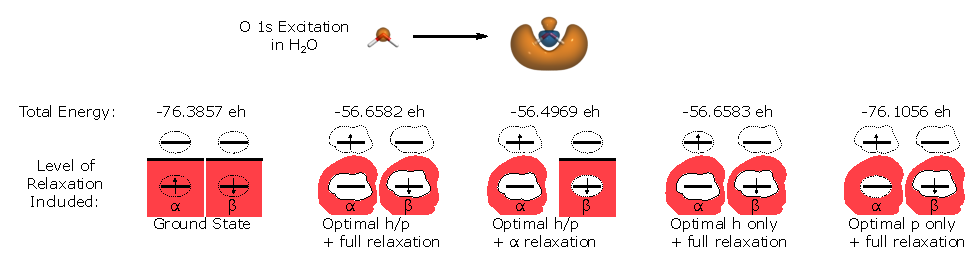
\includegraphics{h_p_algorithms.pdf}
\caption{First O 1s core excitation in H$_2$O calculated using orthogonality constrained density functional theory at the B3LYP/3-21G level of theory. Numbers reported are the total energy of the ground state and respective core excited state calculated with varying degrees of orbital relaxation included.}
\label{fig:relax}
\end{figure}
Figure \ref{fig:relax} shows the results of applying these different levels of relaxation to the first core excited state in H$_2$O. Optimizing the hole and particle pair with full relaxation yields a total energy of $- 56.6582$ Hartree. Only relaxing the $\alpha$ orbitals raises this energy by about 0.2 Hartree, showing that the rearangment that occurs in the electronic structure due to the creation of a core hole is significant. This highlights the importance of valence rearrangement and inclusion of hole relaxation effects. The ability of OCDFT to explicitly account for this effect makes it an excellent method for computing core-excitation energies accurately. 
\subsubsection{Stability of the Self-Consistent Algorithm}
The Ritz variational principle defines the energy expectation value $\tilde{E}$ of any trial wavefunction $\tilde{\phi}$ as an upper-bound with respect to the ground state energy $E_0$ of the system
\begin{equation}
\tilde{E} = \frac{\langle \tilde{\phi}| \hat{H} | \tilde{\phi}\rangle}{\langle\tilde{\phi}|\tilde{\phi}\rangle} \geq E_0.
\end{equation} 
However, the energy of a variationally computed excited state $E^{\prime}$ is no longer a valid upper bound of the ground state energy unless the trial wavefunction ($\tilde{\phi}$) is constrained to be orthogonal to all lower lying states of the same symmetry. In this regard, a standard $\Delta$SCF calculation of an excited state can be viewed as an unconstrained optimization, which in many cases guides the final optimized excited state solution to the ground state wave function. This is a well known optimization problem called ``variational collapse.'' Considering this issue, it is desirable to have a method that allows for the general variational calculation of an excited state without sacrificing the orthogonality of the computed excited state wavefunction to lower lying states of the same symmetry. Imposing orthogonality constraints into the variational procedure ensures the strict upperboundedness of the computed excited state energies, which ensures that the optimization will not suffer from variational collapse. This is the approach taken by orthogonality constrained density functional theory as well as the ``takes orthogonality constraints into account'' (TOCIA) method.\cite{tsaune_towards_1994} Other methods such as Morokuma's electron-hole potential (EHP) method\cite{morokuma_extended_1972} and the constricted variational DFT method (CV-DFT) of Ziegler et al. \cite{cullen_formulation_2011,ziegler_implementation_2012} aim to avoid this optimization problem without imposing exact orthogonality and instead impose different variational constraints. Despite these differences, all of these methods revolve around the variational minimization a unique KS energy functional for the excited state determinant $\Phi^{\prime}$ that is different from the ground state reference $\Phi$. They do this explicitly by parametrizing the wavefunction using a generic determinant, this can be expressed as a unitary transformation of the ground state determinant
\begin{equation}
|\Phi^{\prime} \rangle = |\phi_1^{\prime}, \phi_2^{\prime}, ..., \phi_n^{\prime} \rangle = e^{\hat{A}}|\Phi\rangle,
\end{equation}
where $\hat{A}$ is a one-particle anti-Hermitian operator. To impose an orthogonality condition on the excited state wavefunction ($\langle \Phi^{\prime}|\Phi\rangle$ = 0) OCDFT imposes the minimal orbital orthogonality constraints necessary to obtain an orthogonal solution. For example, to provide a description of the lowest excited state, the ground state HOMO ($\phi_n$) is simply constrained to be orthogonal to the excited state occupied orbitals ($\phi_i^{\prime}$) 
\begin{equation}
\langle \phi_n|\phi_i^{\prime} \rangle = 0, i = 1,2,...,n
\end{equation}
This constraint guarantees that the excited state determinant is orthogonal to the excited state, thus ensuring that the resulting optimization procedure does not suffer from variational collapse. 
\subsubsection{Favorable Computational Cost and Scaling}
A cheap computational cost and favorable scaling with respect to system size are extremely important features of OCDFT that allows for a wide range of potential applications for the method. Formally the cost of OCDFT is identical to that of a ground-state DFT computation which scales as $N^3$ for pure functionals and $N^4$ for hybrid functionals, where $N$ is the number of electrons in the system. This scaling with respect to system size is comparable to that of CIS and TDDFT which also scale as $N^4$, in which the bottleneck in those methods is the contraction of a transition density matrix with the two-electron integrals. This scaling is better than that of ADC(2) and excited state CC2 which scale as $N^5$. Unlike CIS and TDDFT, OCDFT maintains this favorable cost while still obtaining accurate excitation energies comparable to more expensive methods, as will be shown in Chapters 2 and 3 of this dissertation.
\section{Prospectus}
In Chapter 2, we report an extension of orthogonality constrained DFT to compute core excited states and generalize the original formalism in order to calculate multiple excited state solutions. This chapter focuses on benchmarking the method with respect to experimental core excitation energies and simulating full experimental spectra. Chapter 3 reports the combination of OCDFT with a novel implementation of the spin-free exact-two-component (X2C) one-electron treatment of scalar relatavistic effects in order to study the importance of relativistic effects on core-excited states and treat K-edges of transition metal complexes. Chapter 4 describes a new technique for the automated classification of core excited states that utilizes a unique representation of the unoccupied orbitals known as the localized intrinsic valence virtual orbitals (LIVVOs). This new method of classification is integrated with the OCDFT hole/particle orbital formalism here. Chapter 5 deals with the unique case of targeting the K-edge chemisorbed organic molecules. We introduce a subspace projection algorithm into OCDFT in order to specifically target the core excitations of the organic adsorbate, which is not feasible in the bottom-up algorithm described in Chapter 2.

{\footnotesize 
\bibliography{introduction}
\bibliographystyle{achemso}
}
\end{document}